\Chapter{Útvonalkeresés}

\Section{Gráfok ábrázolása}

Az útvonalkereséshez az adatokat gráfokkal kell ábrázolni. A gráfok ábrázolására két adatszerkezet terjedt el. A szomszédsági mátrix, amely tisztán aritmetikai ábrázolású, valamint a szomszédsági lista, amely aritmetikai és láncolt listás ábrázolású \cite{grafabrazolas}.

\SubSection{Szomszédsági mátrix}

Legyen $G = (V,E)$ véges gráf, és $n$ a csúcsok száma. A gráfot $n \times n$-es mátrixszal reprezentáljuk, az oszlopokat és sorokat a csúcsokkal indexeljük (általában $1, \ldots, n$). Egy mező értéke 1, ha a hozzá tartozó oszlop által meghatározott csúcs szomszédja a sor által meghatározott csúcsnak, különben 0, vagyis
$$
C_{i, j} = \begin{cases}
    1, & \text{ha } (i, j) \in E, \\
    0, & \text{ha } (i, j) \notin E. \\
\end{cases}
$$

Az ábrázolásra használt mátrixot \textit{szomszédsági mátrix}nak nevezzük (másnéven \textit{adjacencia} vagy \textit{csúcsmátrix}). Irányítatlan gráf esetén a mátrix szemmetrikus.

% TODO: Ezt majd valamilyen grafikus formában érdemes lehet átszerkeszteni!

\begin{figure}[htb]
\centering
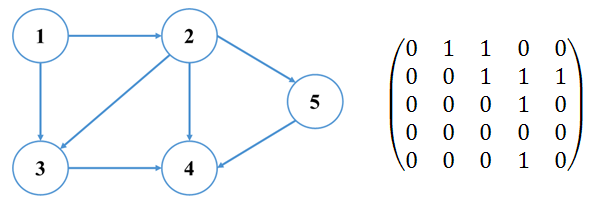
\includegraphics[scale=0.8]{kepek/szomszedsagi_graf_matrix.png}
\caption{Egy irányított gráf és szomszédsági mátrixa}
\label{fig:szomszedsagi_graf_matrix}
\end{figure}

$$
C =
\left(
\begin{array}{ccccc}
0 & 1 & 1 & 0 & 0 \\
0 & 0 & 1 & 1 & 1 \\
0 & 0 & 0 & 1 & 0 \\
0 & 0 & 0 & 0 & 0 \\
0 & 0 & 0 & 1 & 0 \\
\end{array}
\right)
$$

Súlyozott gráf esetén a súlyok tárolása is a mátrixban történik. Ahol az előző megoldásban 1-es található, tehát létezik az adott él, oda az él költsége kerül.

Az ábrázolás helyfoglalása a mátrix méretének négyzetével, vagyis $n^2$-tel arányos, független az élek számától

\SubSection{Szomszédsági lista}

Ennél a módszernél a gráf minden csomópontjához egy listát rendelünk, amik az adott csúcsból kimenő éleket tartalmazzák.

Legyen $G = (V, E)$ véges gráf, és $n$ a csúcsok száma. Felveszünk egy $Adj[1 \ldots n]$ tömböt, amely mutatókat tartalmaz. A tömb indexelése a csúcsokkal történik. A mutatók az éllistákra (szomszédsági listákra) mutatnak.

Irányított gráf esetén az éleket az éllisták listaelemei reprezentálják. A listaelem tárolása abban a listában történik, amelyik csúcsból az él kiindul. A listaelemben a célcsúcs indexét tároljuk. Az $(i, j) \in E$ él az $i$-edik listában egy listaelem, melyben $j$, mint az él célcsúcsa, el van tárolva.

\begin{figure}[htb]
\centering
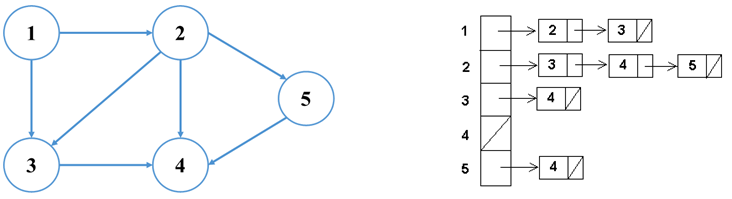
\includegraphics[scale=1.5]{kepek/ellista_iranyitott.png}
\caption{Irányított gráf éllistás ábrázolása}
\label{fig:ellista_iranyitott}
\end{figure}

Irányítatlan gráf esetében egy élnek két listaelemet is megfeleltetünk. Élsúlyozott gráf esetén az él súlyát is a listaelemben fogjuk tárolni.

Az ilyen típusú ábrázolás helyfoglalása irányítatlan gráfok esetében a csúcsok számával ($Adj$ tömb) és az élek számával (az éllista elemeinek a számával) arányos, ami összesen $(n + e)$. Irányított gráfoknál az élszám duplájával kell számolni, azaz $(n + 2e)$-vel arányos a helyfoglalás.

\Section{Útvonalkeresés algoritmusa}

Útvonalkeresés során adott két pont közötti legrövidebb út megtalálása a cél. A legrövidebb út a $G$ gráf adott $u$ csúcsból $v$ csúcsba vezető útjai közül az, amelyiknek a költsége a legkisebb. A költség ez esetben időt jelent, vagyis az úthoz tartozó élek idejét kell összegezni az adott út költségének a meghatározásához \cite{legrovidebbut}.

% \SubSection{Algoritmusok}

A számos útvonalkereső algoritmus közül kettőt szeretnék részletesebben bemutatni, a Dijkstra-, illetve a Floyd-Warshall-algoritmust.

\SubSection{Dijkstra-algoritmus}

Az algoritmust Edsger Wybe Dijkstra, holland matematikus és informatikus fejlesztette ki 1956-ban. Az algoritmussal a legrövidebb utakat lehet megkeresni egy adott csúcspontból indulva irányított vagy irányítatlan gráfokban egyaránt \cite{dijkstra}.

Az algoritmus bemenete egy súlyozott $G$ gráf és a gráf egy $s$ csúcsa. Az út kiinduló pontja az $s$ csúcs. $V$ jelölje a $G$ gráf csúcsainak halmazát, legyen $(u, v)$ a $G$ gráf $u$-t $v$-vel összekötő éle, $u$ és $v$ a gráf csúcsai. $E$ jelölje a $G$ gráf éleinek a halmazát. A $w: E \rightarrow [0, \infty]$ súlyfüggvény az élekhez rendelt súlyokat adja meg, $w(u, v)$ az $(u, v)$ él súlya. Az út költsége két csúcs közt az úton lévő élek összköltsége. Az algoritmus megkeresi a legkisebb költségű $s$-ből $t$-be vezető utat. Ezenkívül arra is alkalmas, hogy adott pontból indulva a gráf minden másik pontjába vezető legrövidebb utat megkeresse.

A $G$ gráf minden $v$ csúcsára nyilvántartja az $s$ és $v$ közötti, a futás során addigi legrövidebbnek megtalált út költségét. Induláskor az $s$ csúcsra ez az érték $0$ ($d[s] = 0$), a gráf összes többi csúcsára pedig végtelen ($d[v] = \infty$) minden $v$-re, kivéve $s$). Ennek az az alapja, hogy kezdetben egy utat sem ismerünk, ami az $s$ csúcsból a többibe vezetne. Az algoritmus lefutása után $d[v]$ az $s$-ből $v$-be vezető legrövidebb út költségét tartalmazza, amennyiben létezik út a két csúcs között. Ha nem létezik, akkor $d[v]$ értéke végtelen marad.

Az algoritmus az $S$ és $Q$ halmazokat használja, amelyekben csúcsokat tárol. Az $S$ halmaz a $G$ gráf azon csúcsait tartalmazza, amelyekre $d[v]$ már az odavezető legrövidebb út költségét tartalmazza. A $Q$ halmazban a gráf többi csúcsa található. Kezdetben az $S$ halmaz üres, majd minden egyes iterációval egy csúcs a $Q$ halmazból az $S$ halmazba kerül. Azt a csúcsot választja ki az algoritmus, amelyiknek a legalacsonyabb a $d[u]$ értéke. Amikor az $u$ csúcs a $Q$ halmazból az $S$-be helyeződik, az algoritmus $u$ összes $v$ szomszédjára megvizsgálja, hogy az addig ismert legrövidebb utak tovább rövidíthetőek-e oly módon, hogy a kezdőpontból az $u$-ig vezető legrövidebb úthoz hozzáadjuk az $(u, v)$ él költségét. Ha az eddig ismert legrövidebb útnál kisebb költséget kapunk, akkor $d[v]$ értéke ez az új, kisebb érték lesz.

Az algoritmus pszeudokódja:

\begin{verbatim}
1  function Dijkstra(Graph, s):
 2     for each vertex v in Graph:     
 3         dist[v] := infinity         
 4         previous[v] := undefined
 5     dist[s] := 0                    
 6     Q := copy(Graph)                
 7     while Q is not empty:
 8         u := extract_min(Q)        
 9         for each neighbor v of u:
10             alt = dist[u] + length(u, v)
11             if alt < dist[v]       
12                 dist[v] := alt      
13                 previous[v] := u
\end{verbatim}

Amennyiben csak az $s$-ből $t$-be vezető legrövidebb útra van szükségünk, akkor a keresést a 9. sorban befejezhetjük, ha $u = t$ teljesül. A legrövidebb út meghatározása:

\begin{verbatim}
1 S := empty sequence
2 u := t
3 while defined previous[u]
4     insert u at the beginning of S
5     u := previous[u]
\end{verbatim}

Ekkor $S$ az $s$ csúcsból a $t$-be vezető legrövidebb utak egyikének csúcsait tartalmazó lista, vagy üres, ha nem létezik ilyen út.

Az algoritmus működését szemlélteti az alábbi egyszerű példa.

\begin{figure}[htb]
\centering
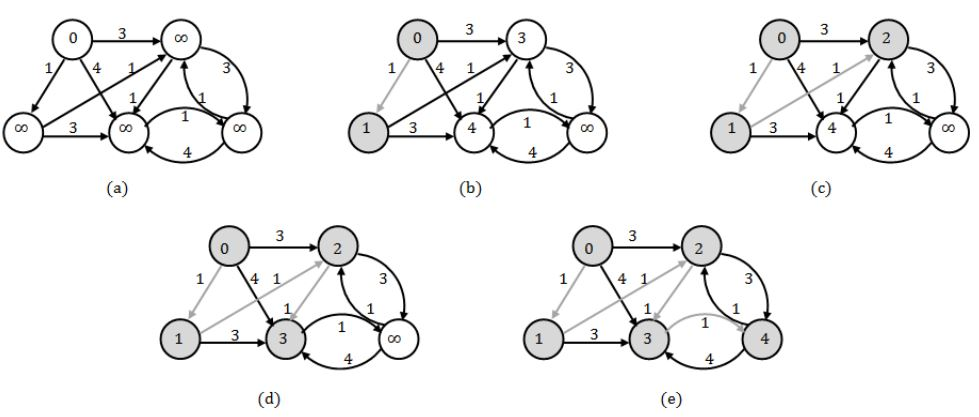
\includegraphics[scale=0.5]{kepek/dijkstra.jpg}
\caption{A Dijkstra-algoritmus működése}
\label{fig:dijkstra}
\end{figure}

\SubSection{Floyd-Warshall-algoritmus}

Két külön algoritmusról van szó, Warshall algoritmusa idősebb a Floyd-algoritmusnál, de a módszerük megegyezik \cite{floyd-warshall}. A szakirodalomban gyakran egyként kezelik a két algoritmust a hasonlóságuk miatt, és Floyd-Warshall néven hivatkoznak rá.
A különbség az algoritmusok közt, hogy a Warshall-algoritmus csak arra ad megoldást, hogy mely pontok közt található irányított út, nem adja meg azok hosszát.

A Floyd-Warshall-algoritmus pszeudokódja:

% TODO: A pszeudó-kódot érdemes lehet kicsit átfogalmazni inkább!
% http://www.uni-miskolc.hu/~matnf/adatst/ea/eaf.ppt

\begin{verbatim}
1 let dist be a |V| x |V| array of minimum distances initialized to oo (infinity)
2 for each vertex v
3    dist[v][v] <- 0
4 for each edge (u,v)
5    dist[u][v] <- w(u,v)  // the weight of the edge (u,v)
6 for k from 1 to |V|
7    for i from 1 to |V|
8       for j from 1 to |V|
9          if dist[i][j] > dist[i][k] + dist[k][j] 
10             dist[i][j] <- dist[i][k] + dist[k][j]
11         end if
\end{verbatim}

Az algoritmus lépésszáma a három egymásba ágyazott for ciklus miatt $n^3$-bel arányos, vagyis $T(n) = \mathcal{O}(n^3)$. Ez nagyságrendben ugyanannyi, mint a Dijkstra-algoritmus mátrixos változata, de a Floyd-módszer 50\%-kal gyorsabb. Amennyiben a gráf éleinek száma kisebb, mint $2n$, és az élsúlyok nemnegatívak, akkor viszont a Dijkstra-algoritmus éllistás változatát érdemesebb használni.

\SubSection{Útvonaltervezés implementálása}

Az elméleti áttekintés után térjünk rá az útvonaltervezés implementációjára. Mivel ez egy viszonylag komplex probléma, így több iterációban történt az implementálás. Először csak a natív, irányítatlan gráfot hoztam létre a GTFS-adatokból, és az ebben való keresésre implementáltam a Dijkstra-algoritmust. Miután ezt sikerült megvalósítani, fokozatosan építettem be a további feltételeket, megszorításokat a gráfgeneráló és az útvonalkereső algoritmusba.

Első változatban a gráfot dictionary-k dic\-ti\-o\-na\-ry-eként hoztam létre. A külső dic\-ti\-o\-na\-ry-ben a kulcsok az egyes megállók nevei, az érték pedig egy másik dictionary. A belső dictionary-ben a kulcsok szintén megállónevek. Jelentésük, hogy a külső megállóból ebbe a megállóba közvetlenül el lehet jutni. Ebben a fázisban azt még nem tartalmazta a gráf, hogy ezt melyik viszonylatokon keresztül lehet megtenni. A belső dictionary-ben az értékek a költséget jelentik, hány másodperc alatt lehet eljutni egyik megállóból a másikba. Ezáltal egy súlyozott, irányított gráf épült fel az adatokból, a súlyozás a másodpercben kifejezett időköltség a két megálló közt.

Egy részlet az így felépített gráfból:

\begin{verbatim}
{
    'AUCHAN Borsod': {'Szondi György utca': 300.0},
    'AUCHAN-dél (Pesti út)': {
        'Pesti út': 60.0,
        'Sütő János utca': 300.0
    },
    'Aba utca': {
        'Zoltán utca': 60.0,
        'Szent Anna tér': 120.0
    },
    'Alföldi utca': {
        'Orvosi rendelő': 60.0
    },
    'Alsó-Hámor': {
        'Felső-Hámor': 60.0,
        'Csanyik-völgy': 60.0
    },
    'Alsó-Majláth': {
        'Felső-Majláth': 120.0,
        'Diósgyőr városközpont': 120.0,
        'Bölcs utca': 60.0,
        'Móra Ferenc utca': 120.0},
    ...
}
\end{verbatim}

Jól látható, hogy az AUCHAN Borsod megállóból egyedül a Szondi György utca megállóba tudunk eljutni, 300 másodperc alatt. Ezzel szemben például az Alsó-Majláth megállóból indulva eljuthatunk 120 másodperc alatt Felső-Majláth, Diósgyőr városközpont és a Móra Ferenc utca megállókba, 60 másodperc alatt pedig a Bölcs utcába.

Miután a gráfgeneráló algoritmust elkészítettem, a Dijkstra-algoritmus implementálása következett.

A függvény három paramétert vár, a gráfot, valamint egy kezdő- és végpontot, tehát két megálló nevét. Először egy ellenőrzés történik, hogy a paraméterként megadott megállók szerepelnek-e a gráfban. Ha igen, megkeresi a legrövidebb utat köztük. Két értékkel tér vissza, a \texttt{path} tartalmazza a kiszámolt utat, a \texttt{cost} értéke pedig az út időköltsége lesz.
Egy példa a függvény meghívására:

\begin{verbatim}
path, cost = dijkstra(graph, 'Balassa utca', 'Vologda városrész')
\end{verbatim}

A függvény által kiszámolt út (\texttt{path} tartalma):

\begin{verbatim}
[
    'Balassa utca',
    'Vasúti sorompó',
    'Vízügyi Igazgatóság',
    'Bajcsy-Zsilinszky út',
    'Búza tér/Zsolcai kapu',
    'Szeles utca',
    'Petőfi tér',
    'Dózsa György út',
    'Vologda városrész'
]
\end{verbatim}

Az eredményt egy listában adja vissza, amely a megállók neveit tartalmazza. A \texttt{cost} értéke pedig 420 ebben az esetben.

Miután ezzel elkészültem, a gráfot kibővítettem, hiszen nem elegendő csak annyit tudni, hogy egy megállóból mely másikakba vezet út. Azt is el kell tárolni, hogy ez a kapcsolat melyik viszonylaton érhető el. Olyan is előfordulhat, hogy A-ból B-be több viszonylaton is el lehet jutni, az optimális útvonal megtervezéséhez ezt is figyelembe kell venni, nem elég csupán egy viszonylatot eltárolni.
Mindezek figyelembevételével átalakítottam a gráf struktúráját. Továbbra is egy dictionary-ről van szó, ahol a kulcsok a megállók nevei, az értékek azonban listák. A listákban dictionary-k vannak, mindegyik dictionary-ben pedig három kulcs-érték pár. A \texttt{name}-hez tartozó érték a megálló neve, a \texttt{cost} a költség, a \texttt{route} pedig a viszonylatot azonosítja.
Részlet a kibővített gráfról:

\begin{verbatim}
{'AUCHAN Borsod': [{
    'name': 'Szondi György utca',
    'cost': 300.0,
    'route': 'AU1'
}],
'AUCHAN-dél (Pesti út)': [{
    'name': 'Pesti út',
    'cost': 60.0,
    'route': '44'
}, {
    'name': 'Sütő János utca',
    'cost': 300.0,
    'route': 'AU2'
}],
'Aba utca': [{
    'name': 'Zoltán utca',
    'cost': 60.0,
    'route': '1'
}, {
    'name': 'Szent Anna tér',
    'cost': 120.0,
    'route': '1'
}, {
    'name': 'Zoltán utca',
    'cost': 60.0,
    'route': '1É'
}, {
    'name': 'Szent Anna tér',
    'cost': 120.0,
    'route': '1É'
}, {
    'name': 'Zoltán utca',
    'cost': 60.0,
    'route': '54'
}, {
    'name': 'Szent Anna tér',
    'cost': 120.0,
    'route': '54'
}], ...
}
\end{verbatim}

Az Aba utca megállóhoz tartozó bejegyzést, ha jobban szemügyre vesszük, könnyen megérthetjük, hogy milyen változás történt. Míg az előző változatban annyi információt tároltunk csak el, hogy a Zoltán utca és a Szent Anna tér megállókba lehet innen eljutni 60 és 120 másodperc alatt ('Aba utca': {'Zoltán utca': 60.0, 'Szent Anna tér': 120.0}), addig a kibővített gráf sokkal több információt tartalmaz. Láthatjuk, hogy mindkét irányba három viszonylaton is (1, 1É, 54) eljuthatunk. Így a gráf mérete a többszörösére növekedett, azonban ez a változtatás elengedhetetlen volt, hiszen az útvonaltervezésnek csak úgy van értelme, ha a viszonylatokat is figyelembe vesszük.

Ezután természetesen az útvonaltervező algoritmust és át kellett írni, hogy kezelni tudja az átalakított struktúrájú gráfot.

Az átalakítás után, az előző példánál maradva, ha kipróbáljuk a Balassa utca és a Vologda városrész megállókkal az algoritmust, akkor a \texttt{path} eredménye a következő lesz:

\begin{verbatim}
[{
    'name': 'Balassa utca', 'route': '3'
}, {
    'name': 'Vasúti sorompó', 'route': '3'
}, {
    'name': 'Vízügyi Igazgatóság', 'route': '3'
}, {
    'name': 'Bajcsy-Zsilinszky út', 'route': '3'
}, {
    'name': 'Búza tér/Zsolcai kapu', 'route': '1'
}, {
    'name': 'Szeles utca', 'route': '1'
}, {
    'name': 'Petőfi tér', 'route': '1'
}, {
    'name': 'Dózsa György út', 'route': '1'
}, {
    'name': 'Vologda városrész', 'route': None
}]
\end{verbatim}

Az eredményt szintén egy listában adja vissza, azonban a listában most már nem csak pusztán a megállók nevei vannak, hanem dictionary-kben név és viszonylat kulcs-érték párok. Jól látható, hogy a Balassa utcából a 3-as viszonylaton elindulva, a Búza tér/Zsolcai kapu megállóban az 1-es viszonylatra átszállva juthatunk el a Vologda városrészbe.
